\PassOptionsToPackage{top=3cm,left=3cm,right=3cm,bottom=3cm}{geometry}
\documentclass[fleqn,11pt]{wlscirep}

\usepackage{import}
\usepackage{main-lancet}

\renewcommand{\paragraph}[1]{\vspace{0.3cm}\noindent\underline{\emph{#1}}\hfill\noindent}

% word count
% \newcommand{\maincount}[1]{%
%   \immediate\write18{texcount -1 -sum=1 -merge -q -nobib #1.tex > #1-words.sum}%
%   \input{#1-words.sum}%
% }

% \newcommand{\abstractcount}[1]{%
%   \immediate\write18{texcount -template="{abst}" #1.tex > #1-words.sum}%
%   \input{#1-words.sum}%
% }

\begin{document}

\doublespacing

\title{\bfseries\LARGE\singlespacing{Air cleaners and respiratory infections in schools: A modeling study using epidemiological, environmental, and molecular data}}

% Alternative title: SARS-CoV-2 transmission in schools based on molecular and epidemiological data: potential effects of mask wearing and air cleaners

% author list
\author[1$\ddag$,2]{Nicolas Banholzer}
\author[2,3]{Philipp Jent}
\author[2,4]{Pascal Bittel}
\author[1]{Kathrin Zürcher}
\author[4]{Lavinia Furrer}
\author[1]{Simon Bertschinger}
\author[5]{Ernest Weingartner}
\author[2,4]{Alban Ramette}
\author[1,6,7]{Matthias Egger}
\author[8]{Tina Hascher}
\author[1*,2]{Lukas Fenner}

\affil[1]{Institute of Social and Preventive Medicine, University of Bern, Bern, Switzerland}
\affil[2]{Multidisciplinary Center for Infectious Diseases, University of Bern, Bern, Switzerland}
\affil[3]{Department of Infectious Diseases, Inselspital, Bern University Hospital, University of Bern, Bern, Switzerland}
\affil[4]{Institute for Infectious Diseases, University of Bern, Bern, Switzerland}
\affil[5]{Institute for Sensors and Electronics, University of Applied Sciences and Arts Northwestern Switzerland, Windisch, Switzerland}
\affil[6]{Population Health Sciences, University of Bristol, Bristol, UK}
\affil[7]{Centre for Infectious Disease Epidemiology and Research, University of Cape Town, Cape Town, South Africa}
\affil[8]{Institute of Educational Science, University of Bern, Bern, Switzerland}


\affil[*]{Corresponding author: lukas.fenner@unibe.ch }


\vspace{1em}

\begin{information}\normalfont

\noindent \textcolor{red}{[list of appendices to be added here later; including STROBE]}

% \noindent\textbf{S1 Appendix:} Includes supplementary text, tables and figures.


% \par
\end{information}

%TC:ignore
\begin{abstract}\normalfont
\noindent\textbf{Background:} Infection control measures can reduce airborne transmission of respiratory infections. Using a multiple-measurement approach, we examined the real-world effectiveness of portable HEPA-air filtration devices (air cleaners) in a school setting.\medskip

\noindent\textbf{Methods:} We collected environmental data (CO$_2$ and particle concentrations), epidemiological data (absences related to respiratory infections), audio recordings (coughing), and molecular data (bioaerosol and saliva samples) over seven weeks during winter 2022/2023 in two Swiss secondary school classes. Using a cross-over study design, we compared particle concentrations, coughing, and the risk of infection with vs without air cleaners.\medskip

\noindent\textbf{Findings:} All 38~students (age 13$-$15 years) participated. With air cleaners, mean particle concentration decreased by 77\% (95\% credible interval 63\%$-$86\%). There were no differences in CO$_2$ levels. Absences related to respiratory infections were 13 with vs 22 without air cleaners, and the risk of infection was slightly reduced (relative risk 0.73, 95\% credible interval 0.44$-$1.18), with a 91\% posterior probability for a reduction. Coughing also tended to be less frequent (posterior probability 93\%). Molecular analysis detected mainly non-SARS-CoV-2 viruses in saliva (50/448 positive). The detection rate was similar with vs without air cleaners. Positive samples in bioaerosols (2/105 positive) and HEPA-filters (4/160~positive) were rare, but spatiotemporal analysis of saliva samples suggested within-classroom transmission.\medskip 

\noindent\textbf{Interpretation:} Air cleaners improved air quality, were associated with less coughing, and showed a potential benefit in reducing respiratory infections. Future studies should examine their cost-effectiveness. Airborne detection of non-SARS-CoV-2 viruses was rare, necessitating further research on the importance of close contact vs long-range airborne transmission.\medskip

\noindent\textbf{Funding:} Multidisciplinary Center for Infectious Diseases, University of Bern, Switzerland.

%This study was funded by the Multidisciplinary Center for Infectious Diseases, University of Bern, Bern, Switzerland. NB, LF, and ME are supported by the National Institute of Allergy and Infectious Diseases (NIAID) through cooperative agreement 5U01-AI069924-05. ME is supported by special project funding from the Swiss National Science Foundation (grant 32FP30-189498).

\par
\end{abstract}

\flushbottom
\maketitle

\vspace{2em}

\vspace{0.5em}

\noindent\textbf{Keywords:} schools, air cleaner, respiratory viruses, airborne transmission, molecular detection
% maximum of 3-5 keywords

\thispagestyle{empty}
\sloppy
\raggedbottom

\newpage

\noindent\textbf{\Large{Research in context}} \medskip

\noindent \textbf{Evidence before this study} \smallskip

\noindent We searched Scopus on October 19, 2023, for all publications from inception using the terms ("air filt" OR "air clean") AND ("infection" OR "transmission"). Several studies have shown that air cleaners reduce particle concentrations in indoor air. Studies also showed that air cleaners effectively removed SARS-CoV-2 bioaerosols. One study reported a lower incidence of SARS-CoV-2 in schools using different ventilation strategies, with or without additional air filtration devices. Several simulation studies have demonstrated the efficacy of air cleaners in reducing the risk of indoor transmission. One real-world study during the COVID-19 pandemic was inconclusive regarding the effectiveness of air cleaners in a school setting. \medskip

\noindent \textbf{Added value of this study} \smallskip

\noindent To date, it remains unclear whether the reduction in particle concentrations with air cleaners also translates into lower risks of respiratory infection. This study used a multiple-measurement approach to estimate the risk of respiratory virus infection in a Swiss school and assessed the effectiveness of air cleaners in a cross-over study design. Schools are particularly important because students spend much of their time indoors and may introduce infections from and into their households. We collected molecular, epidemiological, environmental, and audio data over seven weeks during non-pandemic conditions in winter 2022/2023 in a Swiss school. Air cleaners in classrooms improved air quality (lower particle concentrations), were associated with fewer symptoms (less coughing), and showed a potential benefit in reducing absences related to respiratory infections. We found many respiratory viruses in human saliva samples, mainly adenovirus, influenza B, and rhinovirus. Although airborne detection of viruses was rare, spatiotemporal analysis of students' saliva samples indicated that transmission was likely in school rooms. \medskip

\noindent \textbf{Implications of all the available evidence} \smallskip

\noindent Air cleaners have a tangible positive impact on air quality, significantly reducing particle concentrations. While the individual-level reduction in the risk of respiratory infections due to air cleaners may be relatively modest, the collective benefit at the population level, in terms of reducing illnesses and preventing school absences, is likely to be substantial. Future research should examine the cost-effectiveness and feasibility of implementing air cleaners in school and other communal settings.  
 

\thispagestyle{empty}
\sloppy
\raggedbottom

\newpage
%TC:endignore

\setcounter{page}{1}

\section*{Introduction} 

Transmission of respiratory infections such as SARS-CoV-2 and influenza are difficult to mitigate and control. Person-to-person transmission occurs primarily through the release of respiratory particles containing the viruses. Recently, the focus has been on small respiratory particles called aerosols, which have been found to carry the majority of viruses during respiratory activities\cite{Fennelly2020}. Unlike larger respiratory droplets, which tend to settle quickly, aerosols can remain suspended in the air for several hours and travel long distances\cite{Coleman2022,Wang2020,Heneghan2021}.

Improved ventilation systems are critical for a healthy indoor environment, especially in schools where students spend much of their time indoors during the week, and can reduce the risk of respiratory transmission\cite{Wang2021,Morawska2021}. Portable HEPA-air filtration devices (air cleaners) may be another cost-effective alternative to upgrading ventilation systems. Still, the effects of air cleaners on the transmission of respiratory infections are less clear. Several studies have shown that air cleaners reduce particle concentrations in indoor air\cite{Park2020Build,Buising2022InfContr,Banholzer2023PLoSMed}, which is associated with a reduced risk of respiratory infection and mortality\cite{Gordon2014Resp,Kelly2023Atmos,DeAngelis2021EnvRes}. In line with this, a population-level study reported a lower incidence of SARS-CoV-2 in US elementary schools using different ventilation strategies, with or without additional air filtration devices\cite{Gettings2021}. Although some studies could not find an association between particle concentrations and viral RNA load in airborne samples\cite{Nor2021SciRep,Hanna2023PONE}, recent studies showed that air cleaners effectively removed SARS-CoV-2 from the indoor air\cite{Morris2022,Ueki2022mSphere,Myers2022IndoorAir,Rodriguez2021SOTE}. Simulation studies have further demonstrated the efficacy of air cleaners in reducing the risk of indoor transmission of SARS-CoV-2\cite{Lindsley2021} and other respiratory viruses\cite{Cortellessa2023Build}. However, most simulation studies assume that the detection of RNA equals transmissible virus, despite recent data showing a relevant loss of viral infectivity in respiratory particles over time\cite{Oswin2022PNAS}. To date, it remains unclear whether reducing particle concentrations and removing bioaerosols will reduce indoor transmission of respiratory infections. 

We used a multiple-measurement approach to study the transmission of respiratory viruses under non-pandemic conditions and the effect of air cleaners in schools with a cross-over study design in the winter of 2022/2023. We collected epidemiological data (absences likely related to respiratory infections), environmental data (CO$_2$, particle concentrations), audio recordings (coughs), and molecular data (detection of viruses in bioaerosol and human saliva samples) during a seven-week study period from January to March 2023 in two classes of a secondary school in Switzerland. We determined changes in absences related to respiratory infections, positivity rates of saliva samples, particle concentrations, and coughing.

\newpage

\section*{Methods}

\subsection*{Study setting and design} 

\noindent We collected data in two classrooms of a secondary school (age of students 14-17~years) in the canton of Solothurn, Switzerland, for seven weeks from January~16 to March~11, 2023. Figure~\ref{fig:study-setup} shows the schematic study setup. 

\begin{figure}[!htpb]
    \centering
    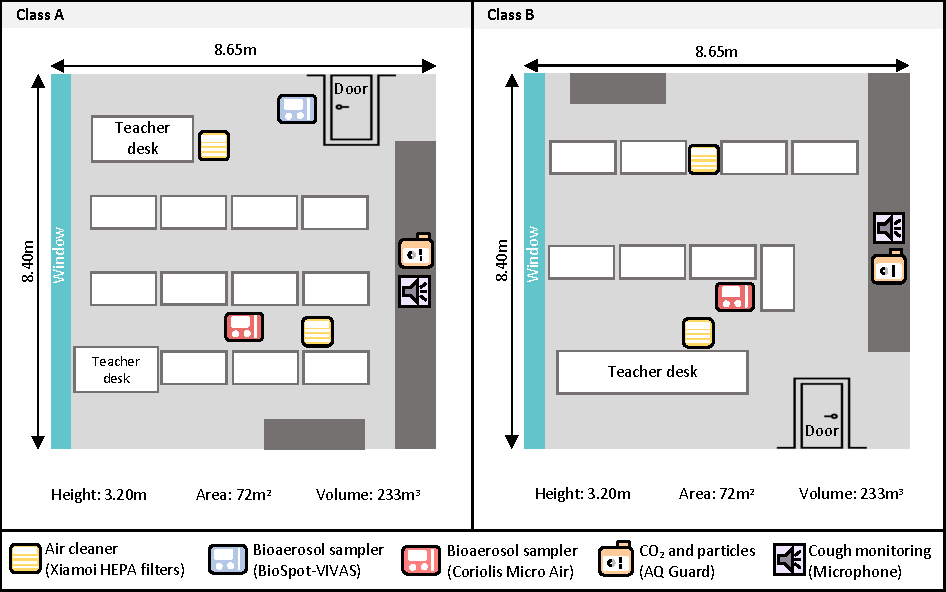
\includegraphics{../study_setting.pdf}
    \caption{\textbf{Study setting}. Schematic study setup of the classrooms. One air cleaner was placed in the front and one in the back of the classrooms. All devices were placed at the head level of the students when they were seated. Both classrooms lacked an active HVAC (Heating, Ventilation, Air conditioning) system, but they were ventilated naturally by opening windows. }
    \label{fig:study-setup}
\end{figure}

\subsection*{Study intervention} 

\noindent We used a cross-over design to study the effectiveness of air cleaners, with two study conditions: weeks with and weeks without air cleaners being installed in each classroom (\cref{tab:study_design}). Air cleaners refer to commercially available portable HEPA-filtration devices (Xiaomi Mi Air Pro 70m², Shenzhen, China). According to the manufacturer, these air cleaners run at clean air delivery rates of 2$\,\times\,$600 m$^{3}$/h. When testing the devices in an empty classroom with sub-micrometer sized particles, we measured a lower effective clean air delivery rate of 2$\,\times\,$420 m$^{3}$/h (\supp~text~\zref{sec:cadr}). Window ventilation was done at the discretion of the teachers.

\begin{table}[!htpb]
    \footnotesize
    \centering
    \caption{\textbf{Cross-over study design.} Description of when portable air cleaners (PAC) were installed in the rooms of classes A and B during a seven-week study period from January~16 to March~11, 2023, excluding a week of vacation from February 6 to 11.}\label{tab:study_design}
    \begin{tabular}{l l l l l l l l l}
    \toprule
      & \textbf{Week 1} & \textbf{Week 2} & \textbf{Week 3} & Vacation & \textbf{Week 4} & \textbf{Week 5} & \textbf{Week 6} & \textbf{Week 7} \\
      & Jan 16-21 & Jan 23-28 & Jan 30-Feb 3 & Feb 6-11 & Feb 13-18 & Feb 20-25 & Feb 27-Mar 3 & Mar 6-11 \\
      \midrule
      \textbf{A} & \cellcolor{gray!50} PAC & \cellcolor{gray!50} PAC\hphantom{000}*& \cellcolor{gray!10} None & & \cellcolor{gray!10} None & \cellcolor{gray!10} None & \cellcolor{gray!50} PAC & \cellcolor{gray!50} PAC\hphantom{0000}* \\
      \textbf{B} & \cellcolor{gray!10} None & \cellcolor{gray!10} None & \cellcolor{gray!50} PAC\hphantom{00000}* & & \cellcolor{gray!50} PAC & \cellcolor{gray!50} PAC\hphantom{000}*& \cellcolor{gray!10} None & \cellcolor{gray!10} None \\
      \bottomrule
      \multicolumn{9}{l}{\scriptsize *~Swabs from the HEPA filters taken after each intervention phase and before the vacation.}
    \end{tabular}
\end{table}
 
\subsection*{Data collection}

An overview of the collected data types is provided in \supp~table~\zref{tab:data}. \medskip

\noindent\textbf{Environmental data} \smallskip

\noindent An air quality device (AQ Guard, Palas GmbH, Karlsruhe, Germany) continuously measured indoor CO$_2$ levels, aerosol number concentrations (particle diameter between 175~nm to 20~$\mu$m) and particle mass concentrations (PM; PM$_1$, PM$_{2.5}$, PM$_4$, PM$_{10}$) by minute. This device was used in previous work\cite{DiGilio2021,Duill2021,Banholzer2023PLoSMed}. The device did \emph{not} alert teachers when CO$_2$ levels or particle concentrations were too high.\medskip

\noindent\textbf{Epidemiological data} \smallskip

\noindent At the beginning of the study, we collected aggregated data on age, sex, COVID-19 vaccination, and COVID-19 recovery status in the participating classes. Daily, we collected data on each absent student, \ie the absence and return dates and reason for the absence (illness, career days, or other). For absences due to illness, we recorded symptoms and the date of symptom onset. We defined a case of respiratory infection as an absence in which the student reported an illness with at least one respiratory symptom (\supp~text~\zref{sec:case-data}). The list of absences by date of symptom onset, absence and return is shown in \supp~table~\zref{tab:epi-data-line-list}.\medskip

\noindent\textbf{Molecular data} \smallskip

\noindent Both classes participated in repetitive bi-weekly saliva testing (Tuesdays and Thursdays; see \nameref{sec:mol_analyses} below). Samples were transported to the laboratory and stored at $-$80°C until further processing\cite{Galar2021,To2019,Huber2021}. The list of positive samples is shown in \supp~table~\zref{tab:mol-data-line-list}. Furthermore, we collected airborne respiratory viruses in both classrooms with a cyclonic bioaerosol sampling device (Coriolis Micro Air, Bertin Instruments Montigny-le-Bretonneux, France), running at 200\,l/min and collecting into 15\,mL Phosphate-Buffered Saline (PBS). The Coriolis Micro Air ran shortly before and during break times (approximately 60\,min/day) to minimize noise. In one class, we also sampled with the BioSpot-VIVAS condensation particle growth collection device (Aerosol Devices Inc., Ft. Collins, CO, USA) \cite{Pan2016JAM,Lednicky2016AST}. BioSpot-VIVAS operated throughout the lessons. The removable parts of both sampling devices were regularly autoclaved. At the end of the day, samples were transported to the Institute of Infectious Diseases (IFIK) and stored at $-$80°C. Finally, we collected swabs from the HEPA filters of the air cleaners after each intervention phase (see \cref{tab:study_design}). The HEPA filters were removed from the air cleaners and divided into 20~fields. One sterile PBS-moistened swab per field was then taken for a total of 20~swabs per filter. \medskip

\subsection*{Laboratory and molecular analyses}\label{sec:mol_analyses}

\noindent Prior to the real-time (RT)-PCR analysis, daily bioaerosol samples were combined for each sampling device and filtered using Amicon Ultra-15 Centrifugal Filters with Ultracel 10,000 Dalton molecular weight cutoffs filters (UFC9010; MilliporeSigma, Burlington, USA) to a volume of 1\,mL. The human saliva samples were analyzed directly without prior filtration. The Allplex RV Master Assay (Seegene, Seoul, South Korea) detects a panel of 19 major respiratory viruses and viral subtypes, including SARS-CoV-2 (CoV), influenza (IF), respiratory syncytial (RSV), metapneumovirus (MPV), adenovirus (AdV), rhinovirus (HRV), and parainfluenza (PIV). 

\subsection*{Molecular genotyping}

We performed molecular genotyping for positive saliva, bioaerosol, air filter samples of adenovirus and influenza. For adenovirus, we used a PCR procedure to amplify three hypervariable regions (hexon, fiber, penton) of the viral genome and then sequenced the PCR products\cite{Akello2021SciRep}. For influenza, we tried to determine the molecular transmission network using whole genome sequencing\cite{Kelly2022FrontiersImmuno}.

\subsection*{Cough detection}

We installed a portable audio recorder (ZOOM H6; New York, USA) in each classroom to record sounds continuously. We determined the number of coughs per minute using an AI algorithm\cite{Bertschinger2023IEEE}. A recent study has shown a significant correlation between coughing and the positivity rate of virus detection in airborne samples\cite{Hanna2023PONE}.

\subsection*{Statistical analyses and modeling}

All statistical analyses were described in a statistical analysis plan (SAP)\cite{Banholzer2023SAP}, which was published prior to the analyses. Contrary to the SAP, bioaerosol samples and viral load concentrations could not be analyzed because there were too few positive samples. Otherwise, there were no major deviations from the SAP. Minor deviations are documented in \supp~text~\zref{sec:transmission-model}-\zref{sec:env-regression-model}, including detailed descriptions of the models. \medskip

\noindent\textbf{Particle concentrations} \smallskip

\noindent We computed mean particle concentrations per day and compared them between study conditions. We estimated the reduction in particle concentrations using Bayesian log-linear regression models, adjusting for class and weekday effects, the number of students in class, the air change rate, and the cumulative number of respiratory cases (\supp~text~\zref{sec:env-regression-model}). \medskip

\noindent\textbf{Risk of infection} \smallskip

\noindent We estimated the relative risk of infection with air cleaners using a Bayesian latent variable hierarchical regression model. The observed outcome of this model is the number of new respiratory cases $C$ (absences related to respiratory infections by date of symptom onset) on day $t$ in class $j$, which are modeled with a Negative Binomial distribution. The expected number of new cases is the weighted sum of the number of new infections $I_{js}$ (unobserved/latent outcome) in the previous days $s<t$, with the weights corresponding to the probability distribution of the incubation period. The number of new infections is related to the presence of air cleaners as follows
\begin{align}
    \log I_{js} = \log F_{js} - \log N_{js} + \beta_0 + \beta_1 \cdot \text{AirCleaner}_{js},
\end{align}
where $F_{js}$ is the number of infections in the previous week (a proxy for the number of infectious students), $N_{js}$ is the cumulative number of infections (a proxy for the number of susceptible students), $\beta_0$ is the infection rate without air cleaners, and $\beta_1$ is the effect of air cleaners. Furthermore, the effect of air cleaners is adjusted for class-specific effects, the number of students in class, the daily air change rate, and the weekly positivity rate for COVID-19 and the consultations for influenza-like illnesses in the canton. A detailed description of the model and choice of priors for all model parameters are provided in \supp~text~\zref{sec:transmission-model}. \medskip

\noindent\textbf{Coughing} \smallskip

\noindent We computed the daily number of detected coughs and compared it between study conditions. We estimated the reduction in the number of coughs using a Bayesian Negative Binomial regression model, using time in class as the model offset and adjusting for class and weekday effects, the number of students in class, the air change rate, and the cumulative number of respiratory cases (\supp~text~\zref{sec:aud-regression-model}). In addition, we used a Bayesian Negative Binomial hierarchical (random effects) regression model to estimate the association between the number of coughs and the number of positive saliva test results. For this analysis, we used only days on which saliva samples were collected (Tuesdays and Thursdays, for a total of 27~days).  \medskip

\noindent\textbf{Saliva samples} \smallskip

\noindent We analyzed the number of positive saliva samples with a Bayesian Multinomial logistic regression model (\supp~text~\zref{sec:multinomial-model}) and linked the expected number of positive samples to the presence of air cleaners, adjusting for the cumulative number of positive tests. \medskip

\noindent\textbf{Software}\smallskip

\noindent All analyses were performed in R software (version 4.2.0)\cite{RCoreTeam2022} and modeling in Stan (version 2.21.0)\cite{Carpenter2017}. Model parameters were estimated with a Bayesian approach, using the Hamiltonian Monte Carlo algorithm with the No-U-Turn Sampler (NUTS)\cite{Hoffman2014}. For each outcome, we report the posterior probability of a reduction with air cleaners. The estimated reduction is reported with the posterior mean and 95\%credible interval (CrI). The code is available from \url{https://osf.io/38j9g}.


\subsection*{Ethics statement}

\noindent The Ethics Committee of the canton of Bern, Switzerland, approved the study (reference no. 2021-02377). For the saliva samples, we included all students who were willing to participate and obtained written informed consent from their caregivers.

\subsection*{Role of the funding source}

The funder of the study had no role in study design, data collection, data analysis, data interpretation, or writing of the report.


\newpage

\section*{Results}

The study population consisted of 38~students (19~female, 19~male; Table~\ref{tab:cases-overview-school}). Seven~students had been vaccinated or recovered from a SARS-CoV-2 infection within the last four months. During the seven-week study period (total of 1,330 student-days), students were absent from school for 220~days (18\% of the total) of which 129~days (59\% of absences) were due to illness.  

\begin{table}[!htpb]
    \centering
    \caption{Overview of the study population and person-days of absences.}
    \label{tab:cases-overview-school}
    \footnotesize
    \renewcommand{\arraystretch}{1.5}
    \begin{tabular}{l r r r}
    \toprule
         &  Class A & Class B & Total \\ \midrule 
        \textbf{Students} & \textbf{20 (53\%)} & \textbf{18 (47\%)} & \textbf{38 (100\%)} \\
        \emph{Gender} \\
        $\drsh$ Female & 11 (55\%) & 8 (44\%) & 19 (\hphantom{0}50\%) \\
        $\drsh$ Male & 9 (45\%) & 10 (56\%) & 19 (\hphantom{0}50\%) \\
        \emph{Immunity status} \\
        $\drsh$ Recently vaccinated (or recovered) & 7 (39\%) & 0 (0\%) & 7 (\hphantom{0}18\%) \\
        $\drsh$ Not recently vaccinated (or recovered) & 11 (61\%) & 20 (100\%) & 31 (\hphantom{0}82\%) \\
        \textbf{Absent person-days} & \textbf{110 (50\%)} & \textbf{110 (50\%)} & \textbf{220 (100\%)} \\
        $\drsh$ Sickness & 52 (47\%) & 77 (70\%) & 129 (\hphantom{0}59\%) \\
        $\drsh$ Other & 58 (53\%) & 33 (30\%) & 91 (\hphantom{0}41\%) \\
        \bottomrule
    \end{tabular} 
\end{table}

\subsection*{Air quality}

The mean aerosol number concentration was 95\,1/cm$^3$ (standard deviation [SD] 81\,1/cm$^3$) without vs 27\,1/cm$^3$ (SD 34\,1/cm$^3$) with air cleaners (\cref{fig:infection-risk}a). The Bayesian regression model suggested a clear reduction in the aerosol concentration with air cleaners, with a posterior probability of 100\%. The estimated decrease was 76\% (95\%-CrI 63\% to 86\%), which was greater for larger than for smaller particles (\supp~figure~\zref{fig:palas-results}). There was little change in other environmental variables (\supp~figure~\zref{fig:env-descriptives-other-vars}). In particular, daily mean CO$_2$ levels were 1,769\,ppm (SD 391\,ppm) with and 1,636\,ppm (SD 341\,ppm) without air cleaners, suggesting that ventilation was comparable between study conditions.

\begin{figure}[!htpb]
\centering
    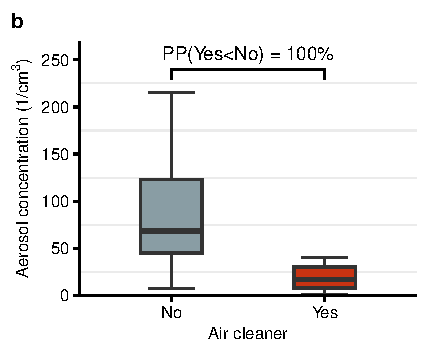
\includegraphics{../../results/env-data/aerosol-number-boxplot.pdf}\hspace{.5cm}
    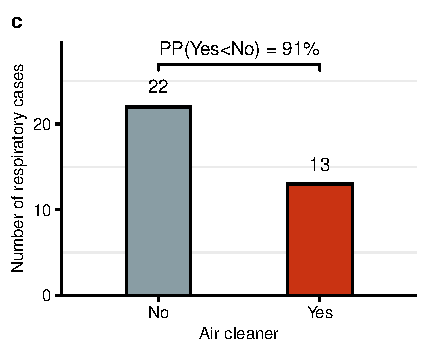
\includegraphics{../../results/epi-data/cases_by_condition.pdf}
    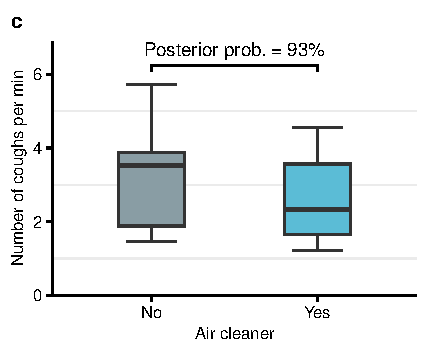
\includegraphics{../../results/cough-data/coughs-frequency-by-condition.pdf}\hspace{.5cm}
    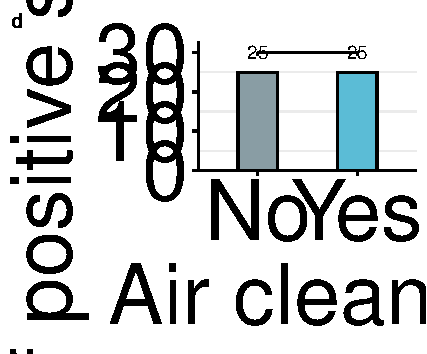
\includegraphics{../../results/mol-data/saliva-by-study-condition.pdf}
    \caption{\textbf{Comparison of outcomes with vs without air cleaners.} At the top of each plot, the posterior probability for a reduction with air cleaners is shown, based on the Bayesian model. \textbf{(a)}~Daily average aerosol number concentrations as boxplots. \textbf{(b)}~Number of respiratory cases. \textbf{(c)}~Daily average number of detected coughs per minute as boxplots. \textbf{(d)}~Number of positive saliva samples.}
    \label{fig:infection-risk}
\end{figure}

\subsection*{Risk of infection}

Absences related to respiratory infections included 22~cases without vs 13~cases with air cleaners (\cref{fig:infection-risk}b). The Bayesian latent variable hierarchical regression model suggested that air cleaners reduced the risk of infection, with a posterior probability of 91\%. The adjusted relative risk of infection with air cleaners was 0.73 (95\%-CrI 0.44 to 1.18). Detailed estimation results are provided in the \supp~text~\zref{sec:detailed-redcap}. 

\subsection*{Coughing}

On average, we detected 3.1\,coughs/min (SD 1.2\,coughs/min) without vs 2.6\,coughs/min (SD 1.1\,coughs/min) with air cleaners (\cref{fig:infection-risk}c). The Bayesian model suggested that coughing was less frequent with air cleaners, with a posterior probability of 93\%. The adjusted relative risk of coughing with air cleaners was 0.93 (95\%-CrI 0.85 to 1.02). Coughing was also associated with virus-specific transmission (\supp~figure~\zref{fig:coughing-association}).

\subsection*{Saliva samples}

We analyzed a total of 448~saliva samples. We detected 15~influenza B, 15~rhinovirus, 14~adenovirus, 3~SARS-CoV-2, 2~metapneumovirus, and 1~parainfluenza virus, respectively (\cref{fig:molecular-descriptives}a). There were 25~positive saliva samples in both study conditions (\cref{fig:infection-risk}d) and, based on the Bayesian model, the posterior probability that air cleaners reduced the positivity rate was 65\%, with an adjusted relative risk of 0.93 (95\%-CrI 0.49 to 1.61; PP 65\%). This estimate was not sensitive to infection to testing delays (\supp~figure~\zref{fig:mol-estimation-results-sensitivity}). 

\subsection*{Transmission patterns}

The distribution of positive saliva samples varied between classes. For example, all but one sample was positive for adenvovirus in class~A during the first three study weeks, while the vast majority of positive influenza~B samples were found in class~B. To illustrate possible transmission chains within classes, we linked positive saliva samples of the same virus that were less than one week apart. Based on this spatiotemporal analysis, we identified 10~possible transmission chains (\cref{fig:molecular-descriptives}b). The longest potential transmission chains occurred in January, referring to a cluster of adenovirus infections in class~A and influenza~B infections in class~B. Molecular genotyping to verify the proposed transmission network was unsuccessful because we could not amplify and sequence any of the gene targets. Furthermore, the rate of positive bioaerosol samples was low. We analyzed 105~bioaerosol samples and detected in two of them viral RNA (1~rhinovirus in class~A and 1~adenovirus in class~B). Similarly, we detected 1~influenza~B, 1~rhinovirus, 1~adenovirus, and 1~SARS-CoV-2 in the 20~swabs taken from each filter of an air cleaner after each intervention phase (160~swabs in total). 

%Nevertheless, these estimates are subject to unmeasured confounding because the delay may be sample-specific and repeated positive tests from the same person could not be precluded because testing was anonymized.

\begin{figure}[!htpb]
    \centering
    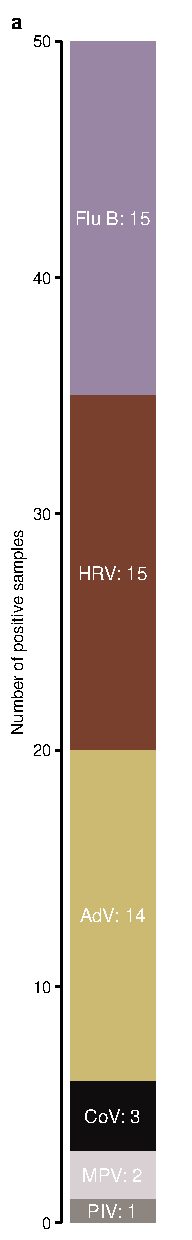
\includegraphics{../../results/mol-data/saliva-distribution.pdf}\hspace{.5cm}
    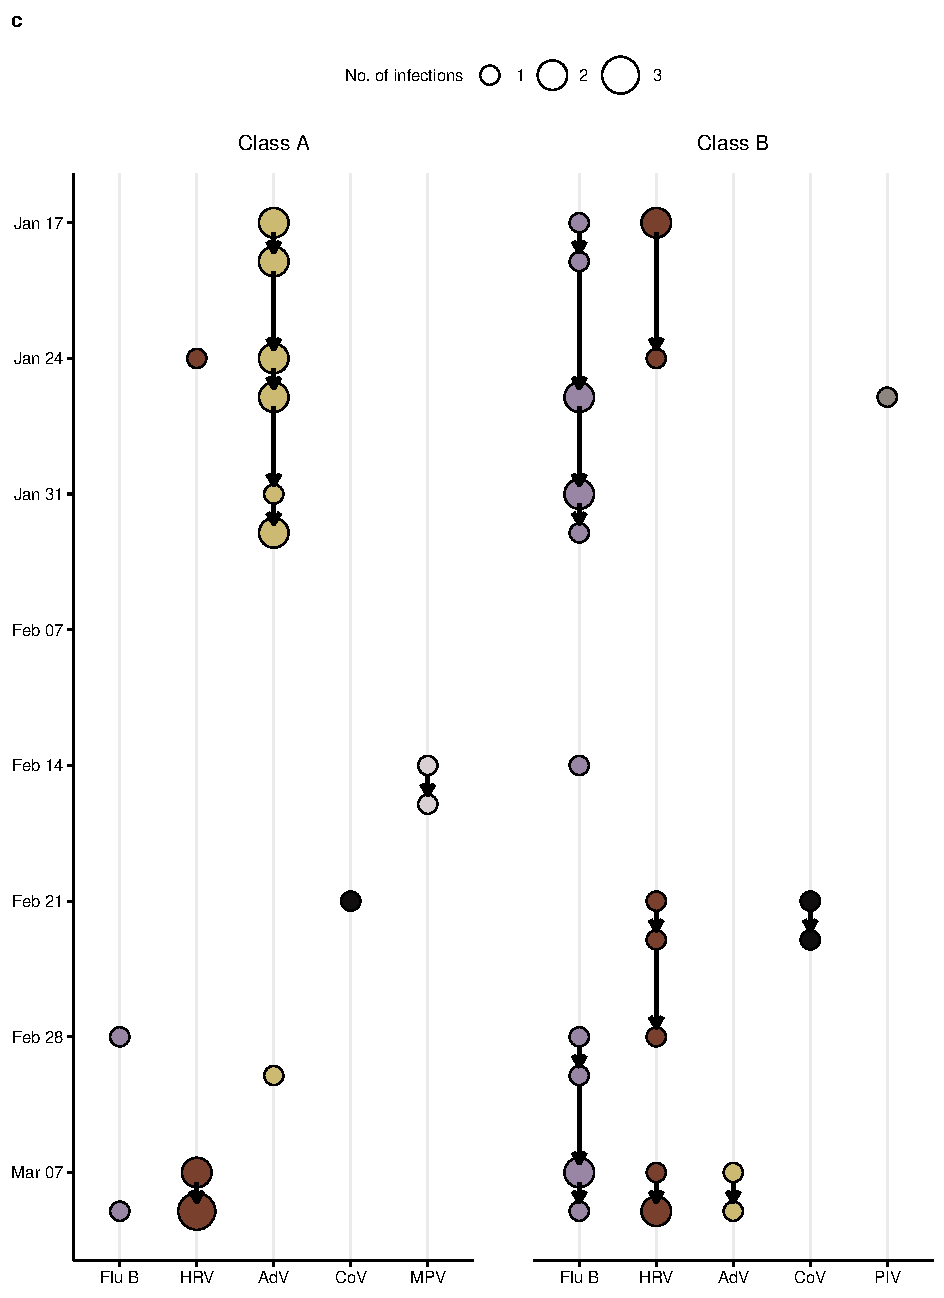
\includegraphics{../../results/mol-data/network-plot.pdf}
    \caption{\textbf{Molecular detection of respiratory viruses and transmission network based on spatiotemporal analysis of students' saliva samples}. \textbf{(a)}~Number of positive saliva samples by virus. \textbf{(b)}~Daily number of positive saliva samples (colored circles) and possible transmission chains within classes (directed arrows). Positive samples are linked if they belong to the same virus and are less than 1~week apart. Positive samples from the air and filters as blank squares aligned. IFB: influenza~B, HRV: human rhinovirus, AdV: adenovirus, CoV: SARS-CoV-2, MPV: human metapneumovirus, PIV: parainfluenza virus.}
    \label{fig:molecular-descriptives}
\end{figure}

\FloatBarrier

\newpage

\section*{Discussion}

% summary

We used a multiple-measurement approach within a cross-over design to estimate the risk of respiratory virus infection in a Swiss school and to assess the effectiveness of air cleaners. We found a wide range of respiratory viruses in saliva samples, mainly adenovirus, influenza B, and rhinovirus, but very few viral RNA were detected in bioaerosol samples and on the filters of the air cleaners. Aerosol number and particle mass concentrations decreased significantly with air cleaners, and Bayesian modeling based on epidemiological data indicated a reduction in the relative risk of infection with air cleaners. Coughing was reduced, compatible with air cleaners preventing some symptomatic infections.

% comparison with previous study 

We estimated the effectiveness of air cleaners during the winter of 2022/2023 in a cross-over design. We detected a range of respiratory virus in students' saliva, mainly adenovirus, influenza~B and rhinovirus, with only three positive SARS-CoV-2 saliva samples. A similar shift in the pattern of respiratory viruses has been observed in other studies\cite{Nygaard2023Lancet,Sauteur2022EuroSurv}. We found a potential benefit of air cleaners on the risk of respiratory infection. In a previous, similar study in the same setting\cite{Banholzer2023PLoSMed}, we estimated the effectiveness of mask wearing and air cleaners during the SARS-CoV-2 omicron wave in the winter of 2021/2022. At that time, we detected almost exclusively SARS-CoV-2 in the students' saliva. We found a reduction in the risk of SARS-CoV-2 infection for mask wearing, but not for air cleaners, possibly because the air cleaners were introduced only at the end of the study, when most students were already infected with SARS-CoV-2. 

% discussing the effect of air cleaners

It is well documented that air cleaners improve indoor air quality\cite{Park2020Build,Buising2022InfContr,Banholzer2023PLoSMed}. There are several reasons why the effect of air cleaners is probably smaller than universal mask wearing, which has been shown to be a very effective infection control measure\cite{Banholzer2023PLoSMed,Heinsohn2022,Gettings2021,Leung2020NatMed,Milton2013PLoSPathogens}. Unlike masks, air cleaners cannot prevent transmission outside the classroom or transmission due to close range, high particle density. Prolonged and close contact may be necessary for transmission of some respiratory viruses\cite{Leung2020NatMed,Brankston2007LancetID} or make transmission more likely despite prior vaccination or infection\cite{Lind2023NatCommun}. Evidence from this and our previous study\cite{Banholzer2023PLoSMed} further suggests that air cleaners are more effective at removing larger particles ($>5\mu$m), which also explains the difference between our measured and the manufacturer's reported clean air delivery rate (see \supp~text~\zref{sec:cadr}). However, many respiratory viruses are carried in smaller particles, which are more relevant for transmission ($\leq5\mu$m)\cite{Fennelly2020}. Finally, classroom activity, airflow and other unobserved, confounding factors make it challenging to evaluate the effects of air cleaners on transmission in real-world settings. Nevertheless, it is important to evaluate their effectiveness in such settings and to compare them with the hypothetical effects suggested by simulation studies\cite{Lindsley2021,Cortellessa2023Build}.

%Although the risk reduction effect estimated in this study is rather small, the cumulative impact may be relevant because minimizing the risk of transmission of respiratory infections in schools is an important public health consideration\cite{Beale2023JOMT} and because prevention and control measures in schools, such as air cleaners, must be adequate and acceptable\cite{WHO2020SchoolMeasures}.

% economic and psychological impact of air cleaners

The beneficial effects of air cleaners on indoor air quality and transmission come at a reasonable cost. The portable air cleaners used in our study cost approximately USD\,250 per unit. Their operating cost effectiveness in providing clean air could be even higher than that of a ventilation system when compared in parallel using the same air delivery ratings\cite{Noh2016EnBuild}. Therefore, air cleaners could be a cost-effective public health measure, particularly during pandemics or epidemics when there is greater exposure to respiratory infections. In addition, air cleaners can have a psychological impact. On the one hand, they can give students and teachers a sense of support during difficult times. For example, it has been shown that getting infected was one of the main worries for students during the pandemic\cite{Yuerekli2022IJERPH}. A safe and supportive environment is a key determinant for students' success and well-being in school\cite{Kutsyuruba2015RevEduc}. On the other hand, air cleaners may not be well accepted by teachers and authorities due to noise, limited space, technical issues, and the required maintenance\cite{Sanguinetti2022IndoorAir}. Therefore, investments in professional building ventilation systems are still preferred in the long term\cite{Nardell2016}.

% transmission within classroom

We detected only few respiratory viruses in bioaerosol samples (1~sample of adenovirus and 1~sample of rhinovirus) and on the filters of the air cleaners (4~positive samples in 160~swabs). The low rate of positive bioaerosol samples may indicate that it is unlikely that airborne transmission occurred to a considerable extent in the classrooms, \ie it is possible that students had relatively little exposure to respiratory viruses at school and acquired their infections elsewhere. However, the distribution of positive saliva samples markedly differed between classes. Adenovirus spread in class~A during the first three study weeks, with only two infections of influenza~B over the study period. In contrast, influenza~B spread throughout the study in class~B, and adenovirus infections were detected only in the last week of the study. Adenovirus infections tend to be mild\cite{Kunz2010CIDR} and less frequently associated with cough than influenza\cite{Ma2018RMV}, which is consistent with the comparatively lower frequency of coughing in class~B. Taken together, the class-specific, spatiotemporal patterns in the spread of respiratory viruses indicate that transmission of respiratory infections may have occurred within the classrooms. 

% limitations

Our study has several limitations. Aerosol measurements and molecular detection of viruses in bioaerosol samples document exposure, but not transmission and the direction of transmission (person to air, air to person) cannot be determined. Further, the reasons for school absences were self-reported by students and some absences may have been incorrectly attributed to respiratory infections. In addition, we could only approximate the incubation period for each epidemiological case. Finally, the study was conducted in two classrooms of one Swiss school and although results are likely to apply to many settings in Switzerland and other European countries, they will not be applicable to settings in the global South. 

% conclusion

In conclusion, using epidemiological, environmental, and molecular data, our study showed that a wide range of respiratory viruses, but rarely SARS-CoV-2, was detected in students under non-pandemic conditions when public health measures were lifted, and that transmission of these respiratory viruses likely occurred in schools. Airborne detection of non-SARS-CoV-2 respiratory viruses was rare, suggesting that that respiratory viruses other than SARS-CoV-2 may be more difficult to detect in the air and that close contact may be required for transmission in most cases. Air cleaners improved air quality by significantly reducing particle concentrations. The reduction in risk of respiratory infections conferred by air cleaners may be modest at the individual level, however, the benefit at the population level in terms of illness and school absences prevented will likely be important. Future studies should investigate the relative importance of prolonged close contact and long-range transmission of respiratory viruses in schools and other congregate settings, and examine the cost-effectiveness of using air cleaners in these settings.

\newpage

%TC:ignore

\section*{Author contributions}
Conception and design: NB, KZ, LF, PB, PJ, TS. Epidemiological and environmental data collection: EW, NB, PJ, KZ, TS, LF. Laboratory data collection: PB, LFu. Additional data collection: TH. Cough detection: SB. Molecular genotyping: AR, PB, LFu. Statistical analysis: NB. Paper draft: NB, LF, ME. All authors reviewed and approved the final version of the manuscript.

\section*{Acknowledgements}
We would like to thank the schools, teachers, and students participating in the study. We are grateful to the Educational Department of the canton of Solothurn for their support throughout the study. We would also like to thank Ronald Dijkman for the influenza molecular genotyping and the biosecurity team (Julia Feldmann, Monika Gsell, Kathrina Summermatter) from the Institute for Infectious Diseases at the University of Bern for their assistance with the bioaerosol devices. Finally, we are indebted to the student assistants (Khadija Ahmed, Marie-Joséphine Brancato, Michelle Bürki, Santiago Martinez, Moric Toszeghi, Sylvain Wasmer) who helped with the data collection in the schools.

\bibliography{references.bib}
%TC:endignore

\end{document}
